\documentclass[10pt,twocolumn,letterpaper]{article}
\usepackage[review]{cvpr}
\usepackage{graphicx,booktabs,multirow,amsmath,amssymb,xcolor,enumitem,xspace}
\usepackage{microtype}
\usepackage{caption}
\captionsetup{font=small,labelfont=bf,skip=4pt}
\newcommand{\todo}[1]{{\color{red}[#1]}}
\newcommand{\pithree}{$\pi^3$\xspace}
\newcommand{\dathree}{DA3\xspace}
\newcommand{\vggt}{VGGT\xspace}
\newcommand{\auc}{AUC@3\xspace}
\newcommand{\wl}[2]{#1/#2}          % significant wins / losses
\newcommand{\sig}{\ensuremath{^{\ast}}}
\newcommand{\mixsize}{r_{\mathrm{s}}}
\renewcommand{\paragraph}[1]{\vspace{2pt}\noindent\textbf{#1}\hspace{0.4em}}

\definecolor{cvprblue}{rgb}{0.21,0.49,0.74}
\usepackage[pagebackref,breaklinks,colorlinks,allcolors=cvprblue]{hyperref}
\usepackage[capitalize]{cleveref}
\crefname{section}{Sec.}{Secs.}
\Crefname{section}{Section}{Sections}
\crefname{table}{Tab.}{Tabs.}
\crefname{figure}{Fig.}{Figs.}

\def\paperID{*****}
\def\confName{CVPR}
\def\confYear{2027}

\title{Views or Pixels? How Feed-Forward 3D Models Fail on Mixed-Resolution Input,\\and How to Spend a Token Budget}
\author{Anonymous CVPR submission\\\\Paper ID \paperID}

\begin{document}
\twocolumn[{%
\renewcommand\twocolumn[1][]{#1}%
\maketitle
\vspace{-1.6em}
\begin{center}
  \centering
  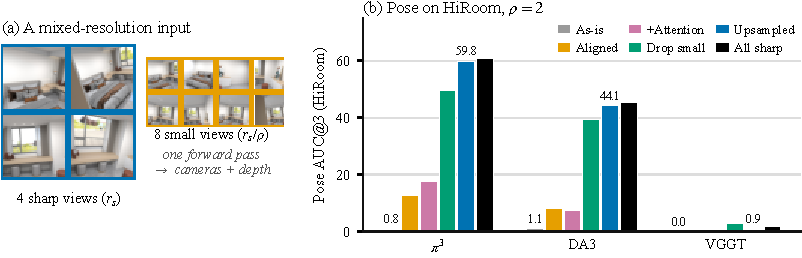
\includegraphics[width=\textwidth]{figures/fig_teaser.pdf}
  \captionof{figure}{\textbf{Mixed-resolution input breaks feed-forward 3D models, and for two of them the loss is mostly not missing information.} (a) One HiRoom scene given as 4 sharp views and 8 views at half resolution. (b) Pose accuracy (\auc, higher is better) over 19 HiRoom scenes. Fed as it is, the mix collapses for all three models. Aligning positions or correcting attention inside the model recovers a little. Upsampling the small views adds no information, yet brings \pithree and \dathree close to the result with all 12 views sharp. VGGT stays low at this token level whatever the input (\cref{sec:diagnosis}).}
  \label{fig:teaser}
\end{center}
\vspace{0.8em}
}]
\begin{abstract}
Feed-forward multi-view 3D models such as VGGT, \pithree and Depth Anything~3 turn every image patch into a token, so their cost is set by how many tokens they are given. An appealing way to spend a fixed budget is to keep a few views sharp and shrink the rest, and inputs of mixed resolution also arise on their own, from camera rigs and photo collections. We study how these three models handle such input on five datasets, using interventions that each change one factor while the frames stay fixed, with every design and prediction written down before its experiments ran. All three models collapse. For \pithree and \dathree the loss is mostly not missing information: upsampling the small views adds no detail, yet recovers 62--110\% of the lost pose accuracy. \dathree, whose global attention gives every patch the same position, collapses as hard as the others, so misaligned positions across views cannot be the whole cause. Corrections inside the model recover little, while resizing every view to one size within the mix's own token cost recovers most of the loss. VGGT behaves differently: it suffers from uneven detail across views, and we do not establish why. Finally, when the budget can be spent freely, the reconstruction gains of mixed inputs come from their extra views. Against uniform inputs with as many views, the best mixes win 6 and lose 11 of 54 comparisons, so a uniform input with the right number of views is the better default.
\end{abstract}

\section{Introduction}
\label{sec:intro}

Feed-forward multi-view models now recover cameras and geometry from a set of images in a single forward pass~\cite{wang2024dust3r,leroy2024mast3r,wang2025vggt,wang2025pi3,lin2025da3}. VGGT~\cite{wang2025vggt}, \pithree~\cite{wang2025pi3} and Depth Anything~3 (\dathree)~\cite{lin2025da3} share one design: each view is cut into $14{\times}14$ patches, each patch becomes a token, and attention alternates between tokens of the same view and tokens of all views. The number of tokens therefore sets the cost of a run, and a practitioner with a fixed budget has to decide how to spend it: on more views, or on more pixels per view.

One answer looks especially efficient. Most of a scene can be covered by a few sharp views, with the remaining views shrunk to save tokens. Inputs of this kind also appear without anyone choosing them, when a rig combines cameras of different resolution or when photos come from different devices. Either way the model receives views of different sizes in one forward pass.

We find that the three models handle this poorly. On HiRoom, \pithree reaches 60.9 \auc when all 12 views are sharp. If 8 of those views are instead given at half resolution, accuracy falls to 0.8 (\cref{fig:teaser}). For pose, the small views can even do harm. When we score only the four sharp frames that every input shares, the mix, even with its positions aligned, is below the four sharp views alone in 28 of 30 settings, 17 of them significantly, and significantly above them in one. A mixed input is therefore not a cheaper version of a sharp one. It is a different kind of input, and the models are not built for it.

This paper asks why, and what a practitioner should do about it. We give each scene a fixed set of frames and change one factor at a time (\cref{fig:arch}). Small views can be fed as they are, with their positions mapped onto the sharp grid, with a correction to their attention, upsampled back to the sharp size, or replaced by sharp versions of the same frames. Upsampling is the key control: it adds no information, but it makes the small views look like sharp ones to the model. If upsampled views recover the loss, the loss came from how the views are represented, not from what they contain. We run the three models on five datasets, for pose and for reconstruction, at two token levels and several resolution ratios. Each study had a written protocol with predictions, fixed before any of its jobs ran. Configurations were chosen on one random seed and every reported number comes from another, a held-out dataset was never used for any choice, and the core diagnosis was repeated on a third seed with new frames. Predictions that failed are reported as failed.

Three findings come out of this.

\noindent\textbf{The failure is mostly about representation, for two of the three models.} For \pithree and \dathree, upsampling the small views recovers 62--110\% of the lost pose accuracy, although it adds nothing the small views did not already contain. \dathree gives every patch the same position in global attention, yet collapses as hard as the others, so misaligned positions across views cannot be the whole explanation. VGGT behaves differently: real detail matters to it, and so does uneven detail across views. We narrow its cause but do not establish it.

\noindent\textbf{Fixing the input works better than fixing the model.} Mapping positions onto a common grid and rescaling attention help, but recover only a small part of the loss. Resizing all views to one size, within the same token cost as the mix, recovers most of it for \pithree and \dathree.

\noindent\textbf{The appeal of mixing comes from extra views.} When tokens can be allocated freely, the best mixes do beat the best uniform inputs in some reconstruction settings. But the mixes use more views. Against uniform inputs with as many views, they win 6 and lose 11 of 54 comparisons.

\paragraph{Contributions.}
\begin{itemize}[nosep,leftmargin=*]
  \item A controlled study of mixed-resolution input for three feed-forward 3D models, five datasets, pose and reconstruction, resolution ratios from 2 to 4, three ways of splitting sharp and small views, inputs whose small views come in four different sizes, and two token levels.
  \item A diagnosis by interventions that separates lost information from representation, including a control model that rules out cross-view position misalignment as the only cause.
  \item A training-free fix that works at equal token cost, and evidence that in-model corrections do much less.
  \item An answer to the allocation question: the gain often credited to mixing resolutions is a gain from view count. We turn the results into a per-model recipe (\cref{tab:recipe}).
\end{itemize}

\section{Related work}
\label{sec:related}

\paragraph{Feed-forward multi-view reconstruction.}
DUSt3R~\cite{wang2024dust3r} and MASt3R~\cite{leroy2024mast3r} regress pointmaps for image pairs and need a global alignment step to handle more views. VGGT~\cite{wang2025vggt} removed that step by processing all views jointly, alternating attention within each view (frame attention) and across all views (global attention), and predicting cameras, depth and points directly. \pithree~\cite{wang2025pi3} drops VGGT's reference view and makes the network equivariant to the order of the views. \dathree~\cite{lin2025da3} predicts depth and rays from a plain transformer backbone and introduces the benchmark whose datasets and evaluation protocol we use. We study these three models as published, with frozen weights, and ask how they respond when the views of one input differ in resolution.

\paragraph{Making these models cheaper.}
Several works reduce the cost of VGGT-style models at a given input. Good Token Hunting~\cite{goodtoken2026} is training-free: each query attends to a subset of frames, and tokens within a frame are spatially downsampled in selected layers, guided by global-attention entropy. ReDT~\cite{redt2026} trains a model that maps each view onto a fixed number of basis tokens, so the cost of global attention no longer grows with resolution. HD-VGGT~\cite{hdvggt2026} trains a high-resolution branch with a learned feature upsampler on top of a low-resolution VGGT branch. These methods change how tokens are produced or used inside the model. We keep the models fixed and change the input: how a token budget is divided among views and pixels. To our knowledge, none of these works evaluates inputs whose views arrive at different resolutions.

\paragraph{Resolution and positions in transformers.}
Vision transformers trained at one resolution can be adapted to others: FlexiViT~\cite{beyer2023flexivit} trains across patch sizes, NaViT~\cite{dehghani2023navit} packs images of any resolution into one sequence during training, and MSViT~\cite{havtorn2023msvit} chooses a token scale per image region. All three models we study encode positions with rotary embeddings (RoPE)~\cite{su2024roformer}. For language models, training-free methods rescale RoPE positions to reach longer contexts: position interpolation~\cite{chen2023pi}, NTK-aware scaling~\cite{bloc97ntk} and YaRN~\cite{peng2023yarn}. For diffusion transformers that generate several resolutions at once, Wu \etal~\cite{crpa2025} rewrite the RoPE index map so that queries and keys are expressed on one grid spacing, and Jin \etal~\cite{jin2023training} rescale attention to keep its entropy stable when the token count changes. We test the training-free position and attention corrections on mixed-resolution input in \cref{sec:fixes} and find that they help, but recover far less than changing the input.

\section{Experimental setup}
\label{sec:setup}

\begin{figure*}[t]
  \centering
  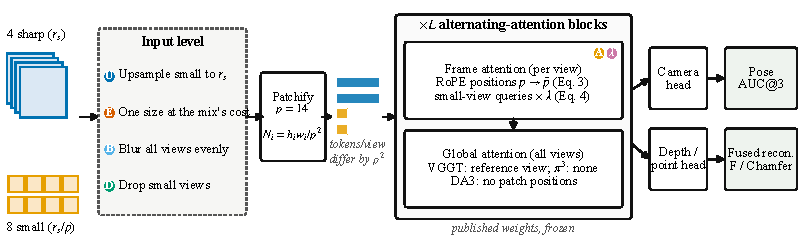
\includegraphics[width=\textwidth]{figures/fig_arch.pdf}
  \caption{\textbf{Where each intervention acts.} The three models share an alternating design: each view is cut into patches, attends within itself (frame attention, with 2D rotary positions), then attends across all views (global attention), and heads predict cameras and depth. In a mixed input, views have different token counts. Input-level interventions (U, E, B, D) change what the model sees. In-model corrections act on frame attention: position alignment (A, \cref{eq:align}) and attention scaling ($\lambda$, \cref{eq:lambda}). The models differ in global attention, which makes \dathree a control for cross-view position effects. Weights stay frozen throughout.}
  \label{fig:arch}
\end{figure*}

\paragraph{Models.}
We use the published weights of VGGT-1B, \pithree and \dathree-Large at pinned code versions, without retraining, in 16-bit floating point. All three use $14{\times}14$ patches. \Cref{tab:models} lists the properties that matter for mixed input. The difference that matters most is in global attention: VGGT and \pithree give each patch its position on its own view's grid, while \dathree gives every patch the same position.

\begin{table}[t]
\centering\small
\setlength{\tabcolsep}{3pt}
\begin{tabular}{@{}lccc@{}}
\toprule
 & VGGT-1B & \pithree & \dathree-L \\
\midrule
Reference view             & first view & none & first view$^*$ \\
Frame-attention positions  & 2D RoPE & 2D RoPE & 2D RoPE \\
Global-attention positions & 2D RoPE & 2D RoPE & shared (none) \\
Default patches $T$        & 1{,}369 & $\approx$1{,}301 & 1{,}296 \\
\bottomrule
\end{tabular}
\caption{\textbf{Model properties relevant to mixed input.} $T$ is the number of patches per view at each model's default input resolution, used in \cref{eq:lambda}. $^*$\dathree chooses its reference view by a configurable strategy; we use the first view.}
\label{tab:models}
\end{table}

\paragraph{Token budget.}
An input of $n$ views, with view $i$ resized to $h_i\times w_i$ pixels, costs
\begin{equation}
  B \;=\; \sum_{i=1}^{n} \frac{h_i\, w_i}{14^2}
  \label{eq:budget}
\end{equation}
patch tokens. Our main budgets are $B{=}4{,}096$ and $8{,}192$, with $2{,}048$ and $16{,}384$ as extensions. A \emph{uniform} input with $n$ views uses the largest resolution at which all $n$ views fit the budget. Tokens are a fair measure of cost here. Timed on one GPU and one scene per dataset, a mix and a uniform input with the same token count differ in run time by $+2\%$ for \pithree, $-2\%$ for VGGT and $+10\%$ for \dathree; some of the timed \dathree mixes include a low-resolution view-selection pass, which adds to their time. Doubling the tokens makes a run 1.5--1.8$\times$ slower, so token counts translate into real cost.

\paragraph{Mixed inputs.}
For the diagnosis, each scene gets 12 views: $n_s{=}4$ sharp views at resolution $\mixsize$ and $n_m{=}8$ small views at $\mixsize/\rho$, with resolution ratio $\rho\in\{2,3\}$. We also test $\rho{=}4$, the splits 2+10 and 6+6, and graded mixes whose 8 small views take four sizes. The lower token level sets $\mixsize$ to the resolution of an 8-view uniform input at 4{,}096 tokens: a long side of 350\,px for 4:3 images and 378\,px for ETH3D, about 470 tokens per sharp view. The higher level uses the 8-view resolution at 8{,}192 tokens: 504\,px and 546\,px, about 1{,}000 tokens per sharp view, which is close to the 518\,px input VGGT uses by default. A seeded shuffle decides which frames are sharp, and all inputs for a scene draw on the same frames.

\paragraph{Interventions.}
Each intervention changes one factor of the mixed input while the frames stay fixed:
\begin{itemize}[nosep,leftmargin=*]
  \item \textbf{As-is}: each view at its own size, with native positions.
  \item \textbf{Aligned}: the small views' rotary positions mapped onto the sharp grid (\cref{eq:align}).
  \item \textbf{+Attention}: aligned, plus an attention correction on the small views (\cref{eq:lambda}).
  \item \textbf{Upsampled}: small views upsampled (bicubic) to the size their image has at $\mixsize$. This adds no information; token count, spacing and positions now match the sharp views.
  \item \textbf{Shrunk}: all 12 views at the small size.
  \item \textbf{One size}: all 12 views at the common resolution $r_{\mathrm{eq}}=\mixsize\sqrt{(n_s+n_m\rho^{-2})/12}$, at which they cost the same as the mix.
  \item \textbf{Blurred}: all 12 views reduced to the small views' resolution and upsampled back, so no view has more detail than the others.
  \item \textbf{Drop}: the 4 sharp views alone.
  \item \textbf{True}: all 12 views at $\mixsize$, the reference.
\end{itemize}
Upsampled against aligned separates representation from information. True against upsampled measures how much real detail the small views lost.

\paragraph{Datasets.}
We use the five datasets of the \dathree benchmark~\cite{lin2025da3}: ETH3D~\cite{schops2017eth3d} (11 scenes), 7-Scenes~\cite{shotton2013scene} (7), ScanNet++~\cite{yeshwanth2023scannetpp} (20), HiRoom (30, of which 19 have at least 12 frames and are used wherever 12 views are needed) and DTU~\cite{jensen2014large} (22). DTU was never used for any configuration choice, so it serves as a held-out test.

\paragraph{Metrics.}
Pose is measured by \auc, the area under the accuracy curve of relative rotation and translation errors up to 3\textdegree, over all pairs of views in the input. On 7-Scenes we use a version that handles the dataset's non-orthonormal ground-truth rotations. Reconstruction fuses predicted depth with predicted cameras, aligns the result to the ground truth with a similarity transform, and reports F-score on the first four datasets and overall Chamfer distance in millimetres on DTU, following the \dathree protocol. All-pair \auc only scores the views an input contains, so inputs with different view counts are scored on different frames. When we compare such inputs, we also score pose on the four sharp frames that every input shares (\emph{common frames}, 6 pairs). We added this control after the first results were read, and say so wherever it is used.

\paragraph{Protocol and statistics.}
Each study had a written protocol that fixed its design, analysis and predictions before any of its jobs ran. Configurations were chosen on a selection seed (42). Every reported number comes from a different seed (1000), which also draws different frames, so no reported number influenced a choice. The core diagnosis was repeated on a third seed (2000) with new frames. Differences are paired by scene and summarised with a 10{,}000-sample bootstrap over scenes. A difference is \emph{significant} when its mean lies more than two standard errors from zero. A \emph{cell} is one model, dataset and setting; we report significant wins and losses over cells as W/L, and the remaining cells are inconclusive. We never pool across budgets, tasks or datasets.

\section{Why the models fail on mixed input}
\label{sec:diagnosis}

\begin{figure*}[t]
  \centering
  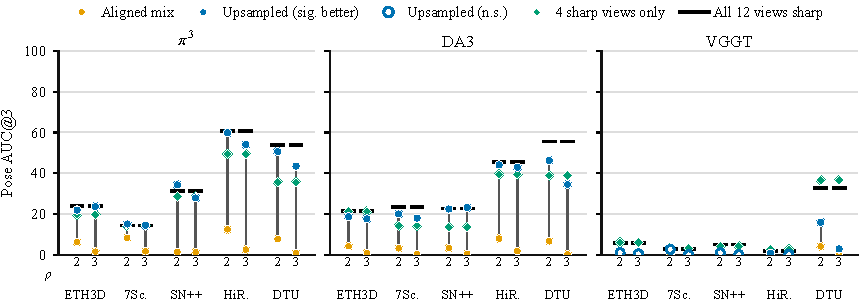
\includegraphics[width=\textwidth]{figures/fig_diagnosis.pdf}
  \caption{\textbf{The diagnosis across all models, datasets and ratios} (pose \auc, 4 sharp + 8 small views, lower token level). For \pithree and \dathree, upsampling the small views (blue) lifts the aligned mix (orange) close to the all-sharp reference (black bar) in every cell, and usually above the 4 sharp views alone (green). For VGGT it does not. Filled blue marks a significant difference between upsampled and aligned.}
  \label{fig:diagnosis}
\end{figure*}

\begin{table}[t]
\centering\small
\setlength{\tabcolsep}{4pt}
\begin{tabular}{@{}lcc@{}}
\toprule
Input (\pithree, HiRoom, $\rho{=}2$) & Pose \auc & F-score \\
\midrule
Mix as-is                        & 0.8  & 0.152 \\
+ positions aligned              & 12.5 & 0.214 \\
+ attention correction           & 17.6 & 0.236 \\
Small views dropped (4 sharp)    & 49.4 & 0.360 \\
Small views upsampled            & 59.8 & 0.699 \\
All 12 views sharp (reference)   & 60.9 & 0.736 \\
\bottomrule
\end{tabular}
\caption{\textbf{One row of the diagnosis.} Upsampling the small views adds no information, yet nearly closes the gap to the all-sharp reference; changes inside the model close little of it. Reconstruction numbers here are from a readout in which not every job had been fused yet (\cref{sec:discussion}).}
\label{tab:teaser}
\end{table}

\subsection{All three models collapse}

\Cref{tab:teaser} follows one setting, \pithree on HiRoom with 8 of 12 views at half resolution, through every intervention. Fed as it is, the mix scores 0.8 \auc against 60.9 when all views are sharp, and its reconstruction F-score drops from 0.736 to 0.152. \dathree falls the same way, from 45.4 to 1.1. VGGT is low with every input at this token level (\cref{fig:teaser}), a point we return to in \cref{sec:vggt}.

The small views are not simply less useful than sharp ones; for pose they can be harmful. When we score only the four sharp frames that every input shares, the aligned mix is below the four sharp views on their own in 28 of 30 pose cells, 17 of them significantly, and significantly above them in one. On the replication seed, dropping the small views again beats the aligned mix on these frames (4/0 for \pithree, 7/0 for \dathree and 4/1 for VGGT). Reconstruction is less one-sided: small views can still add coverage. For \pithree on ETH3D at $\rho{=}2$, the aligned mix reaches an F-score of 0.353 against 0.158 with the sharp views alone.

\subsection{For \pithree and \dathree, the loss is mostly representation}

If the mix fails because small views carry less information, then upsampling them should not help, since it adds none. It helps a great deal. Upsampled small views beat the aligned mix in all 10 pose cells for both \pithree and \dathree (\cref{tab:diag,fig:diagnosis}). The gains are large: $+6.8$ to $+51.5$ \auc for \pithree and $+14.5$ to $+41.0$ for \dathree, and $+0.13$ to $+0.57$ in F-score for \pithree and $+0.12$ to $+0.49$ for \dathree.

To see how much of the loss this recovers, we use the recovery ratio
\begin{equation}
  R \;=\; \frac{\text{up} - \text{aligned}}{\text{true} - \text{aligned}},
  \label{eq:recovery}
\end{equation}
which is 0 when upsampling does nothing and 1 when it matches truly sharp input. For pose, $R$ lies between 80\% and 110\% for \pithree and between 62\% and 102\% for \dathree at the lower token level, and between 87--110\% and 74--104\% at the higher level (\cref{fig:recovery}). Values above 100\% mean the upsampled mix did slightly better than the true sharp input. In other words, giving the small views the same size as the sharp ones recovers most of what was lost, while the information they carry stays the same. For these two models the loss comes mainly from the views being of different sizes, not from what the small views lack.

Real detail does matter at the extremes. The gap between true and upsampled input is concentrated on DTU at $\rho{=}3$, where it is $+10.5$ \auc for \pithree and $+21.1$ for \dathree, and it grows as $\rho$ reaches 4 (\cref{sec:robust}).

\begin{table}[t]
\centering\small
\setlength{\tabcolsep}{2.6pt}
\begin{tabular}{@{}lcccccc@{}}
\toprule
 & \multicolumn{3}{c}{Pose (10 cells)} & \multicolumn{3}{c}{Reconstruction (8 cells)} \\
\cmidrule(lr){2-4}\cmidrule(l){5-7}
First vs second input & \pithree & \dathree & VGGT & \pithree & \dathree & VGGT \\
\midrule
Aligned vs as-is       & 7/0 & 5/0 & 5/0 & 5/0 & 4/0 & 5/0 \\
+Attention vs aligned  & 6/0 & 2/1 & 3/0 & 1/0 & 0/0 & 0/0 \\
Upsampled vs aligned   & \textbf{10/0} & \textbf{10/0} & 3/0 & \textbf{7/0} & \textbf{7/0} & 0/4 \\
Upsampled vs shrunk    & 10/0 & 10/0 & 7/0 & 6/0 & 8/0 & 5/1 \\
True vs upsampled      & 3/0 & 2/0 & \textbf{9/0} & 0/0 & 1/2 & \textbf{7/0} \\
\bottomrule
\end{tabular}
\caption{\textbf{Significant wins/losses of the first input over the second} (4 sharp + 8 small views, $\rho\in\{2,3\}$, lower token level). Pose covers five datasets; reconstruction covers the first four (ETH3D with 9 of 11 scenes). DTU is left out of reconstruction because some of its $\rho{=}3$ inputs have undefined Chamfer distance. VGGT's cells at this level sit close to its floor (\cref{sec:vggt}).}
\label{tab:diag}
\end{table}

\begin{figure}[t]
  \centering
  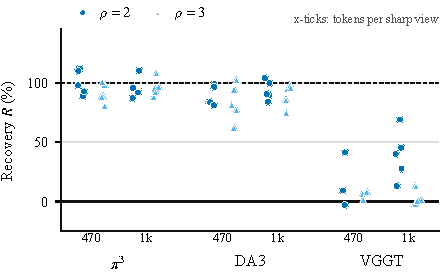
\includegraphics[width=\linewidth]{figures/fig_recovery.pdf}
  \caption{\textbf{Share of the pose loss recovered by upsampling} ($R$, \cref{eq:recovery}), one point per dataset, at two token levels. \pithree and \dathree recover nearly everything at both levels; VGGT does not, even with about 1{,}000 tokens per sharp view. Cells where the all-sharp input beats the aligned mix by less than 3 \auc are omitted, since $R$ is then unstable.}
  \label{fig:recovery}
\end{figure}

\subsection{\dathree rules out positions as the only cause}

Misaligned positions are the obvious suspect. In VGGT and \pithree, a patch of a small view gets a position on its own coarse grid, so in global attention it is compared with sharp-view patches whose positions mean something different. \dathree is a natural control, because its global attention gives every patch the same position. Before running it, we predicted that \dathree would barely degrade on mixed input and that aligning positions would not help it. Both predictions failed. \dathree collapses as hard as the others (1.1 \auc against 45.4 on HiRoom at $\rho{=}2$), and aligning positions, which for \dathree can only act inside frame attention, helps it significantly on all five datasets at $\rho{=}2$. Misaligned positions across views therefore cannot be the whole cause. How many tokens a view has, and how they are spaced, matter within each view as well.

\subsection{VGGT fails differently}
\label{sec:vggt}

VGGT does not follow this pattern. Upsampling beats the aligned mix in only 3 of 10 pose cells, and in reconstruction the aligned mix wins 4 of 8 cells. Real pixels matter instead: true sharp input beats upsampled input in 9 of 10 pose cells and 7 of 8 reconstruction cells.

At the lower token level, VGGT scores close to zero even with all 12 views sharp (on ETH3D at $\rho{=}2$, 5.9 \auc, against 1.0 upsampled), so these cells alone are weak evidence. The higher token level puts VGGT well above that floor: with all views sharp it reaches 54.0 on ScanNet++, against 5.1 at the lower level, and 95.5 on DTU. We predicted that the gap between true and upsampled input would shrink there. It grew in 9 of 10 cells, and upsampling recovers only 13--69\% of the loss at $\rho{=}2$ and between $-3\%$ and 13\% at $\rho{=}3$.

Uneven detail appears to be what hurts VGGT. When all 12 views are blurred to the small views' detail, so that no view is sharper than another, VGGT does better than with 4 sharp and 8 upsampled views in 16 of 20 cells, against 11 of 20 for \dathree and 1 of 20 for \pithree (where the mix wins 2). On ScanNet++ at $\rho{=}2$, the blurred input scores 50.0, close to the 54.0 of all-sharp input, while the sharp-plus-upsampled mix scores 27.3. At $\rho{=}3$ the blur itself costs too much detail (3.9 on the same dataset). VGGT is also far more sensitive to the number of tokens per view: with 10 uniform views on DTU, going from 4{,}096 to 8{,}192 tokens lifts it from 26.2 to 87.2 \auc, against 43.9 to 55.6 for \pithree. VGGT treats its first view as a reference, unlike \pithree, and this is a plausible reason for its behaviour, but we did not test it, and we do not establish why VGGT differs.

\subsection{The diagnosis is robust}
\label{sec:robust}

The picture for \pithree and \dathree holds under every variation we tried, all scored on pose. With splits of 2+10 and 6+6 views, upsampling beats the aligned mix in 20 of 20 cells for both models (VGGT 8 of 20). At $\rho{=}4$ it does so in 10 of 10 for both, and real pixels begin to matter more: the mean gap between true and upsampled input widens from $+2.8$ to $+4.5$ \auc for \pithree and from $+5.6$ to $+9.6$ for \dathree. When the 8 small views come in four sizes ($\mixsize/1.5$, $/2$, $/3$ and $/4$, two views each), upsampling again wins 10 of 10 cells for both models, while for VGGT it wins 1 and loses 2. Finally, we reran the core diagnosis on a new seed, which draws new frames and new sharp views. Of the 189 cells that are significant on both seeds, 188 agree in direction and one flips. On HiRoom at $\rho{=}2$, \pithree's ladder on the new seed reads 0.9 as-is, 9.1 aligned, 57.3 upsampled and 62.7 all-sharp, against 0.8, 12.5, 59.8 and 60.9 on the reporting seed.

\section{What fixes it}
\label{sec:fixes}

\Cref{sec:diagnosis} shows that matching the small views to the sharp ones recovers most of the loss for \pithree and \dathree. Upsampling does this at roughly twice the token cost ($\rho{=}2$) or 2.5 times ($\rho{=}3$), so it is a diagnostic rather than a fix. Here we ask what can be done at no extra cost, first inside the model and then at the input.

\subsection{Corrections inside the model help a little}

\paragraph{Position alignment.}
In a small view, patch $p$ on a grid of $g$ patches per axis sits at a different relative location than patch $p$ on the sharp grid of $g_{\mathrm{ref}}$ patches. We map each small-view position onto the sharp grid,
\begin{equation}
  \tilde p \;=\; \Big(p+\tfrac12\Big)\frac{g_{\mathrm{ref}}}{g} - \tfrac12 ,
  \label{eq:align}
\end{equation}
per axis, so that patch centres cover the same part of the image in both views. Among training-free position policies tested on the selection seed, this ties for best on \pithree: pooled over three datasets, it scores 3.02 \auc, the same as a frequency-split variant, against 3.00 for YaRN~\cite{peng2023yarn}, 2.88 for CRPA-style re-indexing~\cite{crpa2025} and 0.73 for native positions. The best policies differ by at most 0.14 \auc, and none lifts the pooled score above about 3; VGGT stays at its floor under every policy. On the reporting seed, alignment beats the as-is mix in 7 of 10 pose cells for \pithree and 5 of 10 for both \dathree and VGGT, without a loss (\cref{tab:diag}), but on HiRoom it moves \pithree only from 0.8 to 12.5 of the 60.9 that sharp input reaches.

\paragraph{Attention correction.}
A small view has fewer tokens than the model saw in training, which changes how spread out its frame attention is. Following Jin \etal~\cite{jin2023training}, we scale the frame-attention queries of a small view with $N$ patches by
\begin{equation}
  \lambda \;=\; \sqrt{\frac{\log N}{\log T}}\quad (N<T), \qquad \lambda=1 \quad (N\ge T),
  \label{eq:lambda}
\end{equation}
where $T$ is the model's default patch count (\cref{tab:models}). On top of alignment, it helps \pithree in 6 of 10 pose cells without a loss, helps \dathree in 2 and hurts it in 1, and barely changes reconstruction (\cref{tab:diag}). Studies on the selection seed show where its benefit comes from, and two of our predictions about it failed. Its benefit comes entirely from the small views: applied to them alone it gives \pithree a pooled 4.56 \auc, against 2.85 when applied to the sharp views alone. A version calibrated per layer and head to restore attention entropy, fitted on held-out data, kept almost none of the gain, so restoring entropy is not what makes it work. A correction strength chosen on held-out data hurt \pithree on 7-Scenes. Applied to the frozen mixes of \cref{sec:budget}, the correction helps in 4 of 24 pose cells and hurts in 9, mostly for \dathree. We therefore recommend it for \pithree only.

\subsection{Fixing the input works at the same cost}

\paragraph{One size for all views.}
Instead of upsampling, we resize all 12 views to the single resolution $r_{\mathrm{eq}}$ at which they cost exactly as many tokens as the mix. Sharp views lose some detail and small views gain size, but no view differs from another. This beats the aligned mix in 7 of 10 pose cells for \pithree and 4 of 10 for \dathree, with no losses. On HiRoom at $\rho{=}2$, \pithree rises from 12.5 to 42.3 \auc. Real pixels at that same size would give 44.6, and across datasets they add only $+1.4$ \auc for \pithree and $+0.8$ for \dathree on average, so the resized views lose little by being resampled. VGGT is the exception again, with 1 win and 4 losses: at the mix's cost each of its views gets only about 220 tokens, which is too few for it.

\paragraph{Equal detail at the same cost.}
Blurring all views to the small views' detail and then resizing them to one size within the mix's cost beats the aligned mix in 17 of 20 cells for \pithree and 18 of 20 for \dathree, again without losses. For VGGT it wins 3 and loses 5. We predicted that it would help VGGT at the higher token level; at $\rho{=}2$ that prediction held in only 1 of 5 cells.

\paragraph{For pose, fewer views can be better.}
At the mix's cost, the four sharp views alone give better pose than all 12 views at one size in 23 of 30 cells (6 of 10 for \pithree, 8 of 10 for \dathree, 9 of 10 for VGGT), with none the other way; on the four common frames this holds in 20 of 30. \Cref{fig:views} asks how many views to keep. At about 470 tokens per sharp view, fewer views are better; at about 1{,}000, a few extra views help. Over both levels, six views at one size beat twelve in 5 of 20 cells for \pithree (losing 1), 10 of 20 for \dathree and 12 of 20 for VGGT (losing none). Against the four sharp views alone, however, six views mostly lose (W/L of 0/4, 1/5 and 2/11 for \pithree, \dathree and VGGT). The clearest gain is VGGT on DTU, where six views reach 94.9 \auc against 79.5 for four, scored on the common frames; over all pairs the six-view input scores 80.3. We read this as a rule of thumb, about six views at one size when the budget gives each view enough tokens, rather than a fixed optimum.

\paragraph{Shrinking every view.}
A cheaper alternative is to shrink the sharp views to the small size, so all 12 views match at a lower cost. Whether this rescues the mix depends on how large the small views are. At the higher token level, it beats the aligned mix in 7 of 10 cells for \pithree, with no losses; on HiRoom at $\rho{=}2$, 12 small views reach 50.1 \auc with 3{,}072 tokens, against 15.0 for the aligned mix with 6{,}144. At the lower level, where small views are about 175\,px, the result is split (3 wins, 3 losses), and for \dathree and VGGT it does not hold: for VGGT the mix wins all 10 cells at the higher level. Even where shrinking helps \pithree, it gives it more usable views at the price of worse sharp frames: scored on the common frames at the higher level, shrinking loses to the mix in 5 cells and wins in 2. Shrinking never beats the four sharp views alone (0 wins, 53 losses in 60 cells). It is not a general replacement for the other fixes.

\begin{figure}[t]
  \centering
  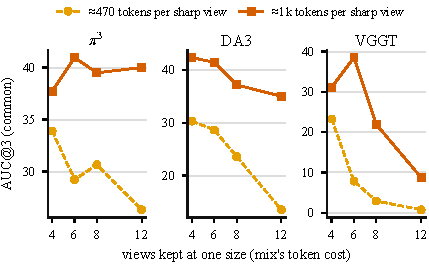
\includegraphics[width=\linewidth]{figures/fig_views.pdf}
  \caption{\textbf{How many views to keep at the mix's token cost.} Pose \auc on the 4 common sharp frames, mean over five datasets ($\rho{=}2$), when the 4 sharp views plus 0, 2, 4 or 8 small views are all resized to one size within the mix's cost. At about 470 tokens per sharp view, fewer views are better; at about 1{,}000, a few extra views help, most clearly for VGGT at 6 views.}
  \label{fig:views}
\end{figure}

\paragraph{Graded mixes.}
The same conclusions hold when the 8 small views come in four sizes. Resizing all views to one size at the mix's cost beats the aligned mix in 9 of 10 cells for \pithree and 7 of 10 for \dathree without a loss, and loses 8 of 10 for VGGT. Twelve views at one size never beat the four sharp views alone for \pithree (0 wins, 3 losses) or VGGT (0 wins, 9 losses), and rarely for \dathree (1 win, 5 losses). Grading the sizes does not create a regime in which mixing pays.

\paragraph{A recipe.}
\Cref{tab:recipe} turns these results into advice for inputs that arrive mixed. For \pithree and \dathree, the best option is to upsample the small views if the budget allows, and otherwise to resize every view to one size. For VGGT, pose is best with the small views left out: on ETH3D the four sharp views score 6.1 \auc against 5.9 for twelve sharp views, and on DTU 36.6 against 32.7. For VGGT reconstruction at $\rho{=}2$, the small views should be kept with aligned positions (F-score 0.166 against 0.113 without them, ETH3D), and at $\rho{=}3$ dropped (0.057 against 0.113).

\begin{table}[t]
\centering\small
\setlength{\tabcolsep}{3pt}
\begin{tabular}{@{}lll@{}}
\toprule
Model & Pose & Reconstruction \\
\midrule
\pithree & Upsample (+ attention) & Upsample \\
\dathree & Upsample & Upsample \\
VGGT     & Drop small views & $\rho{=}2$: keep, aligned; $\rho{\ge}3$: drop \\
\midrule
\multicolumn{3}{@{}l@{}}{\emph{At the mix's token cost:} one size for all views (\pithree, \dathree);} \\
\multicolumn{3}{@{}l@{}}{\quad the sharp views only (VGGT, and pose at low tokens per view).} \\
\bottomrule
\end{tabular}
\caption{\textbf{What to do with an input that arrives mixed.} Derived from the reporting-seed results of \cref{sec:diagnosis,sec:fixes}.}
\label{tab:recipe}
\end{table}

\section{Views or pixels: spending a token budget}
\label{sec:budget}

So far the mix was given. Now suppose the budget can be spent freely. Should one mix resolutions, or use uniform views?

\paragraph{Design.}
For each model and budget, we choose on the selection seed the best uniform input U from a grid of 2 to 32 views, and the best mix X from the mixed inputs of our selection studies. Both choices were frozen before any reporting-seed job ran.

\paragraph{Pose: uniform input wins.}
U beats X in 10 of 24 pose cells, X beats U in 1, and 13 are inconclusive. If mixing paid off where tokens are scarcest, its advantage would grow as the budget shrinks. We predicted this and ran the 4{,}096-token choices at 2{,}048 tokens; the prediction failed. At 2{,}048 tokens, U wins 7 of 15 cells and X none, and on HiRoom \pithree loses 21.6 \auc with the mix.

\paragraph{Reconstruction: the mix seems to help, but because of its views.}
For reconstruction the picture is less clear. X wins 3 cells, loses 3, and leaves 18 inconclusive. On held-out DTU at 4{,}096 tokens, X lowers the Chamfer distance for \pithree from 7.28\,mm to 5.64\,mm and for \dathree from 6.64\,mm to 5.11\,mm; all cells at 8{,}192 tokens are inconclusive. These wins come with a confound. The best mixes use 10 to 12 views, while the best uniform inputs usually use 8. The uniform grid simply had no 10- or 12-view option, so U and X differ in view count as well as in how resolution is spread.

We therefore added uniform inputs with 10 and 12 views at the same budgets (U10, U12) and predicted that they would match or beat the mix, which is what we found. On DTU at 4{,}096 tokens, 12 uniform views reach 5.56\,mm for \pithree, against 5.64\,mm for the mix, and 4.44\,mm for \dathree, against 5.11\,mm. Over all reconstruction comparisons, the mix wins 4 and loses 6 of 30 against U10, and wins 2 and loses 5 of 24 against U12: 6 wins and 11 losses in 54 (\cref{fig:budget}). \Cref{tab:eth3d} shows the clearest case. On ETH3D, \pithree's mix beats the best uniform input from the grid at both budgets, yet 12 uniform views beat the mix by 0.208 in F-score at 8{,}192 tokens. The same holds when the mix's own frames are used: putting all of X's frames at one size, at equal tokens, matches or beats the mix for \pithree (ETH3D at 4{,}096 tokens: the mix is $+0.050$ ahead, not significant; ETH3D at 8{,}192 and HiRoom at 4{,}096: the mix is behind by 0.027 and 0.074, both significant).

\begin{figure}[t]
  \centering
  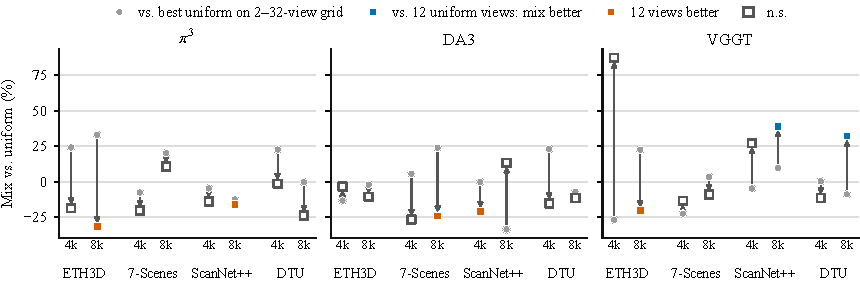
\includegraphics[width=\linewidth]{figures/fig_budget.pdf}
  \caption{\textbf{The mix's reconstruction gain is mostly a gain from extra views.} Relative difference of each model's frozen best mix X against its frozen best uniform input U from the 2--32-view grid (grey circles) and against 12 uniform views U12 (squares; filled when significant, blue = mix better, orange = 12 views better). F-score on ETH3D, 7-Scenes and ScanNet++; negated Chamfer distance on DTU. HiRoom is omitted because 11 of its 30 scenes have fewer than 12 frames. ETH3D uses 9 of 11 scenes.}
  \label{fig:budget}
\end{figure}

\begin{table}[t]
\centering\small
\setlength{\tabcolsep}{5pt}
\begin{tabular}{@{}lcccc@{}}
\toprule
Budget & U (grid best) & X (mix) & U10 & U12 \\
\midrule
4{,}096 & 0.374 & 0.464 & 0.404 & 0.571 \\
8{,}192 & 0.336 & 0.447 & 0.429 & \textbf{0.656} \\
\bottomrule
\end{tabular}
\caption{\textbf{Where mixing seems to pay, more views pay more.} \pithree reconstruction F-score on ETH3D (9 of 11 scenes). The mix X beats the best uniform input from the grid, but not 12 uniform views.}
\label{tab:eth3d}
\end{table}

\paragraph{One exception, and a caution.}
We found one setting where the mix beats every uniform input: VGGT on ScanNet++ at 8{,}192 tokens, with an F-score of 0.364 against 0.332 for U, 0.281 for U10 and 0.262 for U12. Since VGGT needs many tokens per view (\cref{sec:vggt}), the mix may help here by keeping a few views above that threshold. The caution is that pose and reconstruction prefer different inputs: compared with U, the 10- and 12-view inputs give worse pose in 23 of 54 comparisons and better pose in 4. DTU is the exception, where more views also help pose; for \dathree at 4{,}096 tokens, U scores 33.3 \auc and U10 scores 56.1.

\paragraph{Answer.}
When tokens can be allocated freely, the gain people expect from mixing resolutions is, in our results, mostly a gain from using more views. A uniform input with the right number of views is the better default for these models. The right number depends on the task: fewer, larger views for pose, more views for reconstruction.

\section{Discussion}
\label{sec:discussion}

\paragraph{What the results mean.}
Mixed-resolution input is not a cheaper version of sharp input for these models; it is input they handle poorly. For \pithree and \dathree the cause lies mainly in the mismatch of sizes rather than in missing detail, and it is not only a matter of cross-view positions, since \dathree has none. Because the problem sits at the input, the most effective training-free fix is also at the input: give every view the same size. A natural next step is training with mixed-resolution views. Our results suggest what such training would need to cover: views of different token counts within one input, not only lower resolution overall.

\paragraph{Failed predictions.}
Each study's predictions were fixed before it ran, and we report those that failed. \dathree was predicted to barely degrade and to gain nothing from alignment (\cref{sec:diagnosis}). A calibrated attention correction was predicted to improve on the uncalibrated one, and a correction strength chosen on held-out data was predicted to transfer to the other datasets (\cref{sec:fixes}). A corrected mix was predicted to match or beat the best uniform input; it was below it in all 8 cells, 3 of them significantly, which is why this paper studies why mixing fails rather than how to make it win. The mix was predicted to gain at low budgets (\cref{sec:budget}). VGGT's gap between true and upsampled input was predicted to shrink at the higher token level, and equal detail was predicted to help it there (\cref{sec:vggt,sec:fixes}). Shrinking every view was predicted to beat the mix at the higher level for \dathree and VGGT as well as \pithree. Two predictions failed narrowly: twelve views at one size lost to the four sharp views in only 5 of 10 cells for \dathree with graded mixes, and on the replication seed the one-size fix lost one cell for \dathree.

\paragraph{Limitations.}
Our mixes are simulated: small views are downsampled from the same images as the sharp ones. This is what makes a true reference possible, but real mixed captures also differ in sensors, optics and exposure, and ratios beyond 4 or continuous ranges of sizes are untested. We use the published models without retraining. The core diagnosis rests on two frame samples that agree in 188 of 189 cells significant on both; the other studies use the reporting seed only, with the selection seed agreeing in direction. We do not establish why VGGT differs, and its cells at the lower token level sit near its floor. We do not correct for multiple comparisons; no claim rests on a single cell, and our conclusions rest on consistent counts such as 20 of 20. The common-frame scoring was added after the first results were read; it agrees with all-pair scoring. Reconstruction covers fewer settings than pose: ETH3D uses 9 of 11 scenes because two exceed the memory of the fusion step, the studies of splits, ratios, graded mixes, view counts, shrinking and replication are pose only, and apart from the held-out DTU comparison, some reconstruction results come from readouts in which not every job had yet been fused. Cost is measured in tokens, which our timing supports (\cref{sec:setup}).

\paragraph{Conclusion.}
Feed-forward 3D models collapse when the views of one input differ in resolution. For \pithree and \dathree, upsampling the small views restores most of the lost accuracy without adding information, which places the problem in how the views are represented. Corrections inside the model recover little; giving every view one size, at the mix's own cost, recovers most. And when a budget can be spent freely, the benefit often attributed to mixing resolutions turns out to be the benefit of using more views.

{
  \small
  \bibliographystyle{ieeenat_fullname}
  \bibliography{main}
}
\end{document}
